\documentclass[twocolumn]{article}

\usepackage{kotex}
\usepackage{enumitem}
\usepackage{graphicx}
\usepackage{amsmath}
\usepackage{array}
\usepackage{booktabs}
\usepackage{float}
\setlength{\parindent}{0pt}

% Make floats place more readily in this float-heavy two-column draft
\renewcommand{\topfraction}{0.9}
\renewcommand{\bottomfraction}{0.9}
\renewcommand{\textfraction}{0.1}
\renewcommand{\floatpagefraction}{0.85}
\setcounter{topnumber}{3}
\setcounter{bottomnumber}{2}
\setcounter{totalnumber}{5}

\begin{document}

\title{High-throughput LLM Inference on Heterogeneous GPU Clusters through Non-uniform Hybrid Parallelism Planning}
\author{
학번: 2021320057, 이름: 김의찬 \\
지도교수: 서태원 (서명)}
\date{2026.6.18}
\maketitle

\begin{abstract}
Large Language Model (LLM) inference is commonly scaled across multiple GPUs using tensor parallelism (TP), pipeline parallelism (PP), or hybrid combinations of both. Existing serving systems typically assume homogeneous devices and apply uniform partitioning: TP ranks receive equal tensor shards, PP stages receive similar numbers of layers, and the TP/PP degree is selected by simple deployment heuristics. However, this assumption breaks down in heterogeneous GPU clusters, where device compute capability, memory bandwidth, and interconnect characteristics differ significantly. Uniform TP makes the slowest rank a synchronization bottleneck, while uniform PP creates imbalanced pipeline stages and large pipeline bubbles.

This work studies non-uniform hybrid parallelism for LLM inference on a real heterogeneous cluster of eight GPUs spanning two device generations across two nodes. We make three observations. First, the best topology depends jointly on the model \emph{and} the workload phase: across five models and three workloads, a pipelined hybrid layout (TP4$\times$PP2) with skewed layer allocation wins by $+15\%$ to $+155\%$ over uniform TP, but a long-context prefill-heavy 70B workload instead prefers pure non-uniform TP ($+18.5\%$)---``hybrid is not always best.'' Second, naive pipeline parallelism is unprofitable on this cluster because a synchronization gate in the decode path collapses inter-stage overlap to $12$--$24\%$; we identify the gate and restore overlap to $56$--$78\%$ with bit-identical outputs, which is what makes pipelined hybrid layouts win in the first place. Third, non-uniform TP shard ratios and uneven PP layer allocation add a further $+5\%$ to $+25\%$. Building on these, we propose an analytical, workload-aware planner that predicts a near-optimal feasible plan from a roofline cost model and a $\le 6$-cell calibration, without exhaustive online search. On four calibrated models the planner achieves a mean optimality-gap (regret) of $8.5\%$; in a \emph{pre-registered} test it predicted the champion configuration of an unseen 123B model on all three workloads at $0.0\%$ regret before any measurement existed.
\end{abstract}

\section{Introduction}

Large Language Models (LLMs) have rapidly increased in size, making efficient inference a central challenge for modern AI systems. Since many LLMs cannot be served efficiently on a single GPU, inference engines distribute model parameters, activations, and KV cache across multiple devices. Tensor parallelism (TP), pipeline parallelism (PP), and hybrid TP/PP are widely used to scale inference throughput and fit large models into aggregate GPU memory.

Most existing deployments assume that the participating GPUs are homogeneous. Under this assumption, uniform partitioning is natural: each TP rank receives the same number of attention heads and FFN channels, and each PP stage receives approximately the same number of transformer layers. This design is simple, predictable, and effective when devices have similar compute throughput, memory bandwidth, and interconnect performance.

However, real GPU clusters are often heterogeneous. Research labs, universities, and production environments frequently accumulate GPUs across multiple generations or combine servers with different hardware configurations. A single inference pool may therefore include GPUs with substantially different memory bandwidth, FLOPs, memory capacity, and communication topology. The cluster used in this work is a concrete example: four newer high-bandwidth 96\,GB GPUs in one node and four older 48\,GB GPUs in a second node, joined by InfiniBand. In such an environment, uniform model parallelism wastes a large fraction of available resources. In uniform TP, all ranks synchronize after partitioned layer operations; faster GPUs finish early and wait for the slowest rank. In uniform PP, stages with slower GPUs or more expensive layer assignments become pipeline bottlenecks. In hybrid TP/PP, both effects interact: each pipeline stage is bounded by its slowest TP rank, and the overall pipeline is bounded by the slowest stage.

A straightforward remedy is non-uniform tensor parallelism, where faster GPUs receive larger tensor shards and slower GPUs receive smaller shards. This reduces straggler effects inside a TP group. But non-uniform TP alone is not sufficient. LLM inference consists of two distinct phases: prefill and decode. Prefill processes the full prompt and exposes substantial sequence-level parallelism; decode generates tokens autoregressively and repeats the same synchronization-heavy computation for every output token. Because these phases stress hardware differently, the best parallelism strategy depends on workload composition. Decode-heavy workloads often prefer configurations that avoid repeated cross-node synchronization, while prefill-heavy or long-context workloads may benefit from configurations that amortize communication over many tokens.

This observation motivates a broader planning problem. Rather than choosing a fixed TP/PP configuration by rule of thumb, an inference system should plan the full hybrid layout from the hardware profile and expected serving workload. The plan should determine the TP degree, PP degree, per-device TP shard ratio, and per-stage PP layer allocation while satisfying model-architecture constraints such as attention-head grouping and kernel-alignment requirements.

In this work we build a controlled inference engine that supports non-uniform hybrid execution, use it to run a full sweep over five models, four topologies, and three workloads on the heterogeneous cluster, and distill the measurements into an analytical workload-aware planner. This paper makes the following contributions:
\begin{itemize}[leftmargin=*, itemsep=0.2em, topsep=0.3em, parsep=0em]
    \item We show empirically that no single parallelism strategy is best: the champion topology varies with both model and workload phase, and a pipelined hybrid layout wins for most cases but loses to pure non-uniform TP on prefill-heavy 70B (Section~\ref{sec:eval-topology}).
    \item We identify and fix a synchronization gate in the decode path of a production engine that suppresses pipeline overlap to $12$--$24\%$; our fork restores it to $56$--$78\%$ with bit-identical outputs, which is the precondition for hybrid layouts to be competitive (Section~\ref{sec:eval-overlap}).
    \item We implement non-uniform TP (asymmetric attention-head/FFN shards) and uneven PP layer allocation under transformer-architecture constraints, and quantify their $+5\%$ to $+25\%$ benefit (Section~\ref{sec:eval-nonuniform}).
    \item We propose an analytical planner that selects TP degree, PP degree, TP shard ratio, and PP layer allocation from per-device roofline profiles and workload features, and validate it---including a pre-registered prediction on an unseen 123B model at $0.0\%$ regret (Section~\ref{sec:eval-planner}).
\end{itemize}

\section{Background and Motivation}

\subsection{Parallelism for LLM Inference}

LLM inference is constrained by both computation and memory movement. Model weights are read repeatedly, the KV cache grows with sequence length, and each generated token requires a full forward pass. To overcome single-device memory and throughput limits, serving systems distribute inference across multiple GPUs.

\textbf{Tensor parallelism} partitions operations within each transformer layer. For attention, heads or head groups are split across ranks; for FFN layers, intermediate dimensions are partitioned. After local computation, ranks communicate partial results with collectives such as all-reduce. TP reduces per-device memory and increases parallel compute, but it introduces synchronization at \emph{every} layer---two all-reduces per layer in a standard transformer block.

\textbf{Pipeline parallelism} partitions the model by layers. Each GPU group is assigned a subset of transformer layers, and hidden states are passed stage-to-stage with point-to-point messages. PP reduces fine-grained collective communication, but it introduces pipeline dependencies; high utilization requires multiple microbatches in flight, otherwise pipeline bubbles cause stages to idle.

\textbf{Hybrid TP/PP} combines the two: each pipeline stage is a TP group. The design space is therefore the TP degree, PP degree, GPU-to-stage placement, per-rank tensor-shard ratio, and per-stage layer allocation.

\subsection{Heterogeneous GPU Systems}

Heterogeneous clusters violate the assumptions behind uniform partitioning. On our cluster the two GPU classes differ by roughly $2\times$ in effective decode memory bandwidth ($1400$ vs $707$\,GB/s) and $1.6\times$ in effective prefill throughput ($578$ vs $366$\,TFLOPS), and the cross-node InfiniBand link is far slower than intra-node NVLink---a single cross-node all-reduce costs $\approx\!350\,\mu$s.

Under uniform TP, all ranks receive equal shards, so step time is set by the slowest rank; faster ranks idle at every synchronization point. This is especially harmful during decode, where synchronization occurs for every generated token and even small per-token imbalance accumulates over long outputs. Under uniform PP, equal layer counts do \emph{not} imply equal stage latency: a stage on a slower GPU takes longer and limits pipeline throughput. When PP is combined with TP, each stage is further bounded by its slowest rank.

Heterogeneous inference therefore requires hardware-aware parallelism: uneven TP shards within a stage, uneven layer allocation across stages, and workload-aware selection of TP/PP degrees.

\subsection{Why a Single Strategy Is Insufficient}

The reason no single strategy dominates is that prefill and decode expose different bottlenecks. During prefill the model processes many prompt tokens at once: computation is large, sequence-level parallelism is high, and TP all-reduces move large messages that are bandwidth-bound and can be largely hidden behind the GEMMs. During decode the model generates one token at a time: per-step computation is small, all-reduce messages are tiny ($\sim$1--2\,MB) and latency-bound, and on a cross-node TP group the per-step latency floor ($\approx\!2L\cdot\alpha_{\text{cross}}\approx$ tens of ms) dominates. Consequently decode-heavy workloads on this cluster strongly prefer shallow cross-node communication, whereas prefill-heavy workloads can tolerate---and sometimes prefer---wide TP because its communication amortizes over tokens. Heterogeneity sharpens the trade-off: a slow GPU inside a TP group creates rank-level straggling, while a slow pipeline stage creates stage-level bottlenecks. A planner must decide not only \emph{how} to split work unevenly, but \emph{which} form of parallelism should dominate for a given workload.

\section{Problem}

We address the problem of planning model parallelism for LLM inference on heterogeneous GPU clusters. Given a cluster of $N$ GPUs, a transformer with $L$ layers, and an expected serving workload $W=(\textit{in\_len}, \textit{out\_len}, n_{\text{req}})$, the goal is to choose a parallelism plan that maximizes wall-clock throughput subject to model and memory constraints. A plan consists of four interacting choices:
\begin{itemize}[leftmargin=*, itemsep=0.15em, topsep=0.2em, parsep=0em]
    \item the TP degree $M$ and PP degree $K$, where $M \cdot K = N$;
    \item the assignment of GPUs to TP groups and PP stages;
    \item the non-uniform TP shard ratio for attention heads and FFN dimensions;
    \item the PP layer allocation $L_0,\dots,L_{K-1}$ for each stage ($\sum_s L_s = L$).
\end{itemize}

This search space is large, and exhaustively benchmarking every candidate is expensive: each configuration requires model loading, partitioning, warmup, and measurement (minutes per cell). Many candidate splits are also infeasible, because attention heads, KV heads, FFN dimensions, and kernel-aligned matrix shapes impose divisibility constraints, and the smaller-memory rank can run out of KV space at high concurrency. The central challenge is therefore to make non-uniform hybrid parallelism \emph{plannable}: to predict a near-optimal feasible plan from inexpensive profiling and workload statistics rather than online search.

\section{Approach}

Our approach has three parts: a non-uniform hybrid execution engine, a fix that makes pipeline overlap real, and an analytical workload-aware planner with feasibility projection.

\subsection{Non-uniform Hybrid Execution}

We extend a production inference engine's model-parallel path to support uneven work distribution while preserving continuous batching, paged KV cache, and CUDA-graph capture (all experiments keep CUDA graphs on; none use eager mode). For tensor parallelism, attention heads and FFN intermediate columns are assigned per rank according to capability: a faster rank holds more heads and FFN columns, a slower rank fewer. Assignments respect the GQA group as the head quantum and a tensor-core tile ($128$ columns) as the FFN quantum, with a largest-remainder fix-up so shards sum exactly. For pipeline parallelism, transformer layers are allocated unevenly so that the faster node receives more layers. The same engine executes pure TP, pure PP, and hybrid TP/PP, which lets us compare uniform and non-uniform configurations under identical scheduling.

\subsection{Making Pipeline Overlap Real}
\label{sec:approach-overlap}

Pipeline parallelism only pays off when stage $s{+}1$ computes microbatch $i$ while stage $s$ computes microbatch $i{+}1$. In practice we found the stock engine achieved only $12$--$24\%$ overlap during decode, so PP-based layouts were barely competitive. Profiling traced this to the decode path's handling of the sampled token: the previous stage's sampled-token tensor was broadcast on the default CUDA stream, forcing the receiving rank to spin-wait ($\approx\!26$\,ms per microbatch) before launching its own compute, serializing the pipeline.

Our fork moves this broadcast onto a dedicated side stream and replaces the eager wait with a lazy event-wait at the point of use, so the receiving stage overlaps its computation with the broadcast. Combined with disjoint-request microbatching (each microbatch is a distinct subset of in-flight requests, $\textit{mb\_size}\approx n_{\text{req}}/n_{\text{mb}}$, queue depth $bq{=}\textit{pp}$) and a send-side ring buffer, this raises measured overlap to $56$--$78\%$ while producing bit-identical outputs. A lightweight auto-tuner selects $(n_{\text{mb}}, \textit{mb\_size}, bq, \text{broadcast stream})$ from $(n_{\text{req}}, \text{model}, \textit{tp}, \textit{pp})$; its per-request step-time estimates land within $5\%$ of measured.

\subsection{Workload-aware Analytical Planner}
\label{sec:approach-planner}

The planner predicts wall-clock throughput for any candidate $C$ and returns $\arg\max_C \text{TPS}(C)$ subject to memory feasibility, using a roofline cost model rather than learned regression.

\textbf{Per-rank roofline.} For each rank and phase we model the binding resource. Decode is memory-bound: step time is the time to stream the rank's weights plus read its KV slice, $t^{\text{dec}}_r=\max\!\big(\tfrac{P_r b_w}{\text{BW}_r}+\tfrac{\text{KV}_r}{\text{KBW}_r},\,\tfrac{2P_r B}{\text{TF}_r}\big)$, where $P_r$ is the parameter bytes placed on rank $r$. Prefill is compute-bound: $t^{\text{pre}}_r=\max\!\big(\tfrac{2P_r T_c}{\text{TF}_r},\,\tfrac{P_r b_w}{\text{BW}_r}\big)$ for a chunk of $T_c$ tokens.

\textbf{Communication.} A TP stage adds $2L_s$ all-reduces clocked by the \emph{slowest} link in the group: $t_{\text{AR}}=\tfrac{2(N_t-1)}{N_t}\tfrac{\text{msg}}{\text{bw}}+2(N_t-1)\alpha$. This yields two regimes---decode messages are latency-floor bound (the cross-node TP8 killer), prefill messages are bandwidth bound and amortize per token (cross-node prefill all-reduce is $\approx\!80\%$ hidden under the GEMMs).

\textbf{Closed-form optimal splits.} Minimizing $\max_r t_r$ equalizes per-rank time. When attention is fully biasable, the optimum is $\textit{frac}_r^\star=\text{speed}_r/\sum_q \text{speed}_q$ with $\text{speed}_r{=}\text{BW}_r$ (decode) or $\text{TF}_r$ (prefill). When GQA pins heads at full TP (head bias infeasible), only FFN columns are free and we solve a water-filling equalizer over the FFN budget, which predicts the empirically observed $+25$ to $+50\%$ FFN-bias sweet spot as a V-shaped curve bounded below by the unsplittable attention floor. The PP layer split has the analogous closed form $L_s^\star\propto 1/\tau_s$ (per-layer time on stage $s$), refined by a $\pm1$-layer neighborhood search.

\textbf{Pipeline steady state.} With $n_{\text{mb}}$ microbatches in flight the decode cycle is $T_{\text{cycle}}=\max_s t_s+(1-\eta)\sum_{s\neq s^\star} t_s$, where $\eta$ is the measured overlap efficiency ($\eta\!\approx\!0.65$ for our fork, $\eta\!\approx\!0.15$ for stock PP)---directly tying Section~\ref{sec:approach-overlap} to plan quality.

\textbf{Phase blend.} Prefill (tensor-core bound) and decode (HBM bound) run on disjoint resources and partially overlap under chunked continuous batching, so wall time is \emph{not} additive: $T_{\text{total}}=\max(T_{\text{pre}},T_{\text{dec}})+(1-\rho)\min(T_{\text{pre}},T_{\text{dec}})$ with a calibrated overlap factor $\rho$. Modeling the phases as serial blocks over-predicts prefill-heavy wall time by $\sim\!50\%$ and causes spurious topology flips.

\textbf{Feasibility projection and calibration.} The analytically preferred shard may not be executable; the planner projects it to the nearest configuration satisfying head/KV/FFN quanta and rejects (never scores) any plan whose smallest-memory rank exceeds capacity---this reproduces the empirical ``$n_{\text{req}}\!\le\!100$'' limit as a \emph{prediction}. All hardware constants are effective rates fitted from a $\le 6$-cell probe set (per-GPU roofline, intra/cross-node all-reduce, and one PP-overlap pair), making the model portable to a new cluster by direct inversion.

\textbf{Evaluation metric.} Because within-topology layer-skew curves are flat near their optimum (champions win by $<5\%$, comparable to run-to-run noise, and cross-model trends can even disagree), exact top-1 champion match over-fits noise. We therefore report \emph{regret} (the measured throughput lost by deploying the predicted plan instead of the oracle-best) as the primary metric, with Spearman rank-correlation and top-3 hit-rate as secondary, and MAPE for absolute predictor accuracy.

\section{Implementation}

The execution engine is built as a fork of a production LLM serving system (vLLM v1). Non-uniform TP is realized by passing per-rank head/KV/FFN split vectors into the layer construction and collective code; uneven PP is realized by a per-stage layer-partition specification. The overlap fix (Section~\ref{sec:approach-overlap}) touches the decode-time sampled-token broadcast and the microbatch scheduler. The planner is a standalone analytical module ($\sim$1.5k lines) that emits the engine's partition environment variables, so a predicted plan is launched without code changes. The cluster runs across two nodes with Ray, using the InfiniBand interface for both NCCL and the gloo control plane.

\section{Evaluation}

\subsection{Setup}

\textbf{Cluster.} Eight GPUs over two InfiniBand-connected nodes: four high-bandwidth 96\,GB GPUs (effective $578$\,TFLOPS prefill, $1400$\,GB/s decode) and four 48\,GB GPUs (effective $366$\,TFLOPS, $707$\,GB/s). All runs use CUDA graphs (never eager), $\textit{gpu\_mem\_util}=0.85$, and $n_{\text{req}}\le 100$.

\textbf{Models.} Llama-3.1-8B, Llama-3.3-70B (GQA), OPT-30B (MHA), Qwen3-32B, and---for the held-out test---Mistral-Large-2411 (123B).

\textbf{Workloads (input/output tokens).} \textit{decode\_heavy} $128/512$, \textit{balanced} $512/256$, \textit{prefill\_heavy} $1024/128$; $n_{\text{req}}{=}128$ ($96$ for 70B and Mistral, $64$ for OPT-30B).

\textbf{Topologies.} On 8 GPUs we sweep TP8$\times$PP1, TP4$\times$PP2, TP2$\times$PP4, TP1$\times$PP8, each with uniform and non-uniform variants ($15$--$19$ configs per model $\times$ 3 workloads). The baseline is uniform TP8$\times$PP1, the conventional ``just use tensor parallelism'' deployment.

\textbf{Metric.} Wall-clock throughput (total output tokens / wall time), matching the engine's reported \texttt{total\_wall\_throughput\_tok\_s}.

\subsection{The Best Topology Depends on Model and Workload}
\label{sec:eval-topology}

Table~\ref{tab:champion} reports, for each model and workload, the best configuration found across all topologies and its gain over uniform TP8. Two facts stand out. First, the gains are large---up to $+155\%$---confirming that the conventional uniform-TP deployment leaves most of the cluster idle. Second, the winning \emph{family} is consistent but not universal: a pipelined hybrid layout (TP4$\times$PP2 with skewed layers) wins for every model and workload \emph{except} 70B prefill-heavy, where pure non-uniform TP8 with FFN bias wins ($+18.5\%$). This is the concrete sense in which ``hybrid is not always best'': the long-context prefill-heavy 70B case is compute- and bandwidth-bound in a way that rewards wide TP, while every decode-leaning case rewards shallow cross-node communication via PP. Figure~\ref{fig:topology} shows the full topology comparison across models.

\begin{table*}[t]
\centering
\small
\caption{Best configuration per (model, workload) across all topologies, versus the uniform TP8$\times$PP1 baseline. Layer splits are listed as (fast:slow) layers; FFN bias as (fast:slow) intermediate columns. The hybrid TP4$\times$PP2 layout wins everywhere except 70B prefill-heavy.}
\label{tab:champion}
\begin{tabular}{llrlrr}
\toprule
Model & Workload & Baseline TPS & Champion configuration & Champion TPS & $\Delta$\% \\
\midrule
Llama-3.1-8B   & balanced      & 1608 & TP4$\times$PP2 (16:16)            & 3036 & $+88.9$ \\
Llama-3.1-8B   & decode\_heavy & 1726 & TP4$\times$PP2 layer-skew (18:14) & 3887 & $+125.2$ \\
Llama-3.1-8B   & prefill\_heavy& 1503 & TP4$\times$PP2 (16:16)            & 2107 & $+40.2$ \\
Llama-3.3-70B  & balanced      & 1394 & TP4$\times$PP2 layer-skew (44:36) & 1728 & $+24.0$ \\
Llama-3.3-70B  & decode\_heavy & 1468 & TP4$\times$PP2 layer-skew (56:24) & 1683 & $+14.6$ \\
Llama-3.3-70B  & prefill\_heavy& 1155 & \textbf{TP8 FFN-bias (5376:1792)} & 1369 & $+18.5$ \\
OPT-30B        & balanced      & 669  & TP4$\times$PP2 layer-skew (40:8)  & 1301 & $+94.3$ \\
OPT-30B        & decode\_heavy & 676  & TP4$\times$PP2 (24:24)            & 1725 & $+155.1$ \\
OPT-30B        & prefill\_heavy& 557  & TP4$\times$PP2 (24:24)            & 1299 & $+133.1$ \\
Qwen3-32B      & balanced      & 721  & TP4$\times$PP2 layer-skew (48:16) & 1814 & $+151.7$ \\
Qwen3-32B      & decode\_heavy & 743  & TP4$\times$PP2 layer-skew (48:16) & 1834 & $+146.7$ \\
Qwen3-32B      & prefill\_heavy& 730  & TP4$\times$PP2 layer-skew (44:20) & 1744 & $+139.0$ \\
\bottomrule
\end{tabular}
\end{table*}

\begin{figure*}[t]
\centering
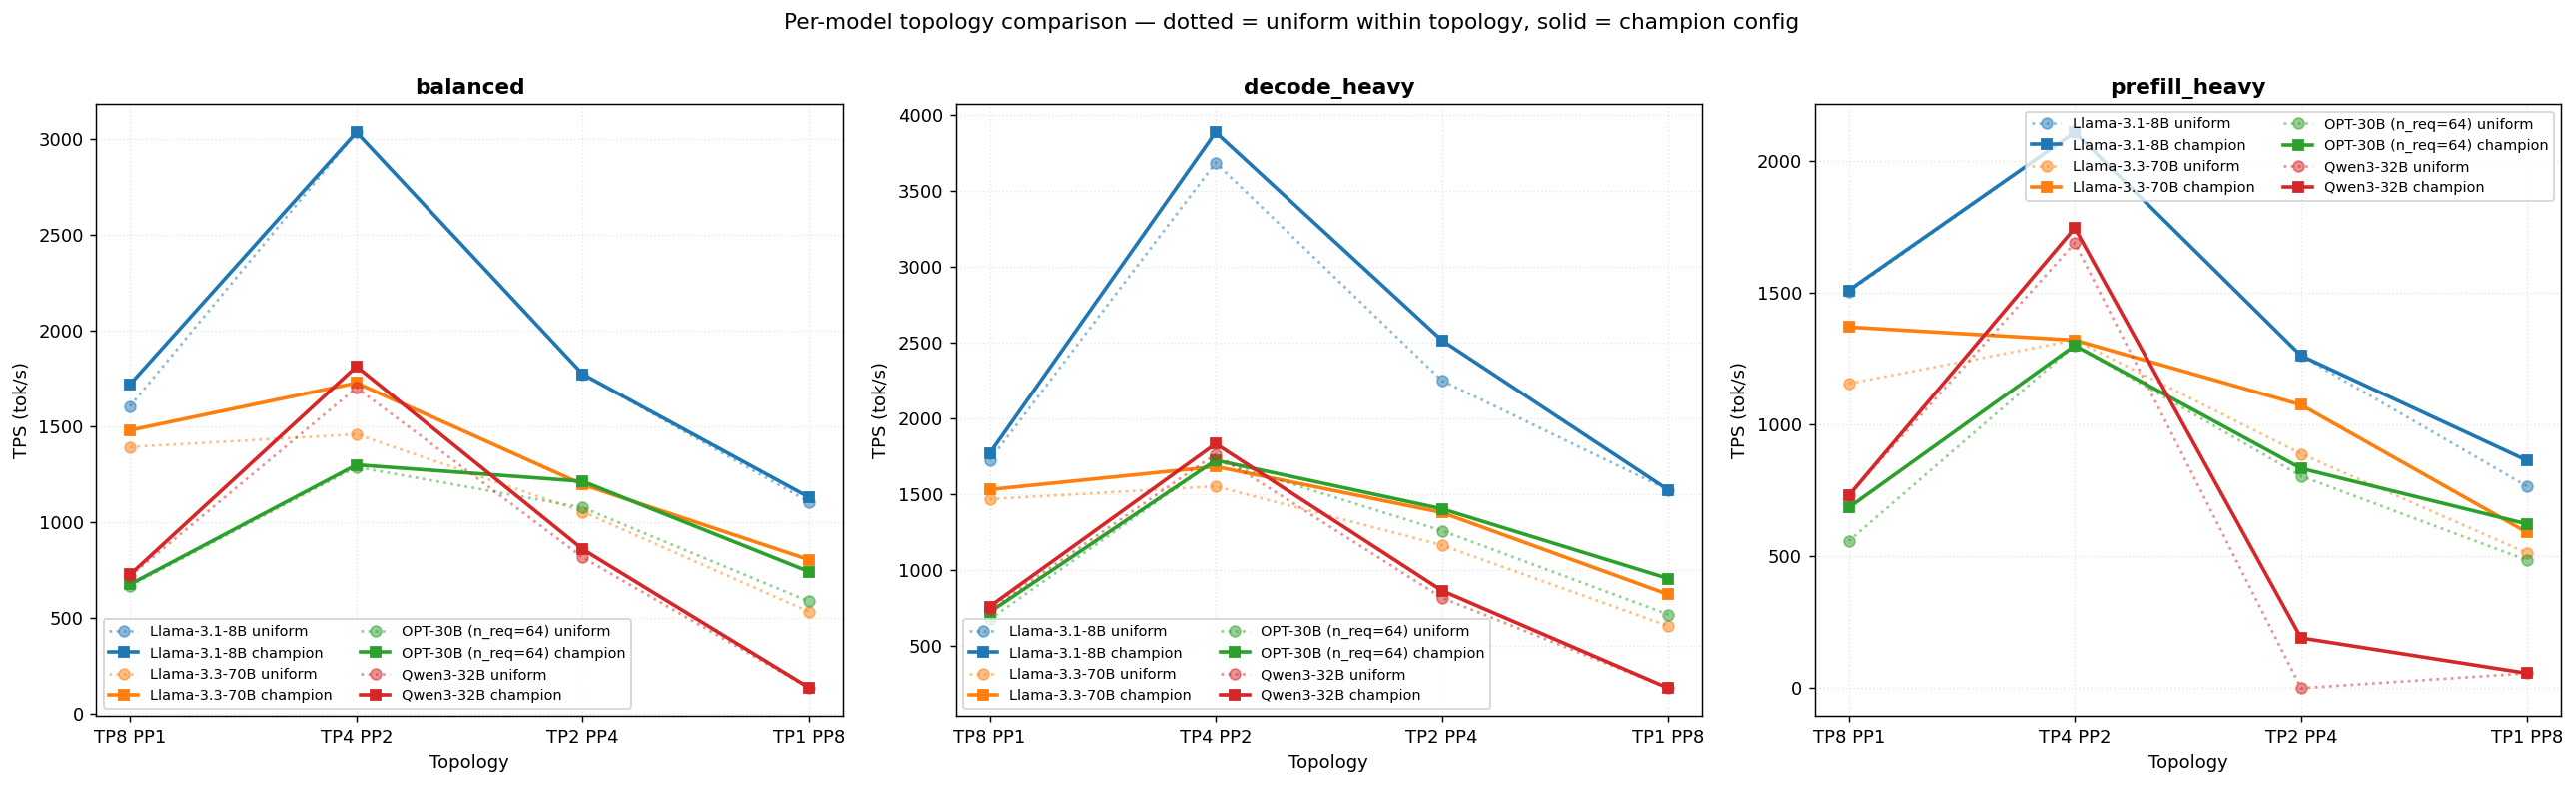
\includegraphics[width=\textwidth]{figures/fig_4model_topology_lines.png}
\caption{Throughput by topology (TP8$\times$PP1, TP4$\times$PP2, TP2$\times$PP4, TP1$\times$PP8) across four models and three workloads. Dotted = uniform partitioning within the topology; solid = best non-uniform (champion) configuration. The pipelined hybrid TP4$\times$PP2 peaks for almost every (model, workload), but the prefill-heavy panel shows a flatter profile where wide TP8 stays competitive (and wins for 70B). The gap between the dotted and solid lines is the non-uniform-partitioning gain.}
\label{fig:topology}
\end{figure*}

\subsection{Pipeline Overlap}
\label{sec:eval-overlap}

The hybrid layouts in Table~\ref{tab:champion} are only viable because pipeline overlap works. With the stock engine, profiling showed inter-stage overlap of just $12$--$24\%$, and PP2 was near parity with TP8 on 70B. After the side-stream sampled-token fix (Section~\ref{sec:approach-overlap}), measured overlap rises to $56$--$78\%$. In an isolated PP=2 decode microbenchmark the fix raises single-stage decode throughput by $2.0$--$2.3\times$; nsight/torch-profiler traces confirm both nodes are simultaneously busy with cross-stage NCCL P2P traffic, and outputs are bit-identical to the stock path.

Table~\ref{tab:overlap} shows the controlled A/B on the 70B uniform TP4$\times$PP2 (40:40) cell: overlap adds $+3.6\%$, $+4.4\%$, and $+9.4\%$ on balanced, decode, and prefill respectively. The gain is larger on prefill (more compute to hide the P2P send behind) and is what lifts TP4$\times$PP2 above uniform TP8 once layer skew is added (Table~\ref{tab:champion}). Figure~\ref{fig:overlap} gives the per-configuration breakdown; we report the uniform cell as the calibrated gain because heavily skewed cells are noisier and can flip sign.

\begin{table}[t]
\centering
\small
\setlength{\tabcolsep}{4pt}
\caption{Stock vs.\ overlap-fixed PP on Llama-3.3-70B, uniform TP4$\times$PP2 (40:40), wall throughput (tok/s).}
\label{tab:overlap}
\begin{tabular}{lrrr}
\toprule
Workload & Stock PP & Overlap PP & $\Delta$\% \\
\midrule
balanced       & 1408.9 & 1459.6 & $+3.6$ \\
decode\_heavy  & 1487.7 & 1552.9 & $+4.4$ \\
prefill\_heavy & 1205.3 & 1319.1 & $+9.4$ \\
\bottomrule
\end{tabular}
\end{table}

\begin{figure}[tb]
\centering
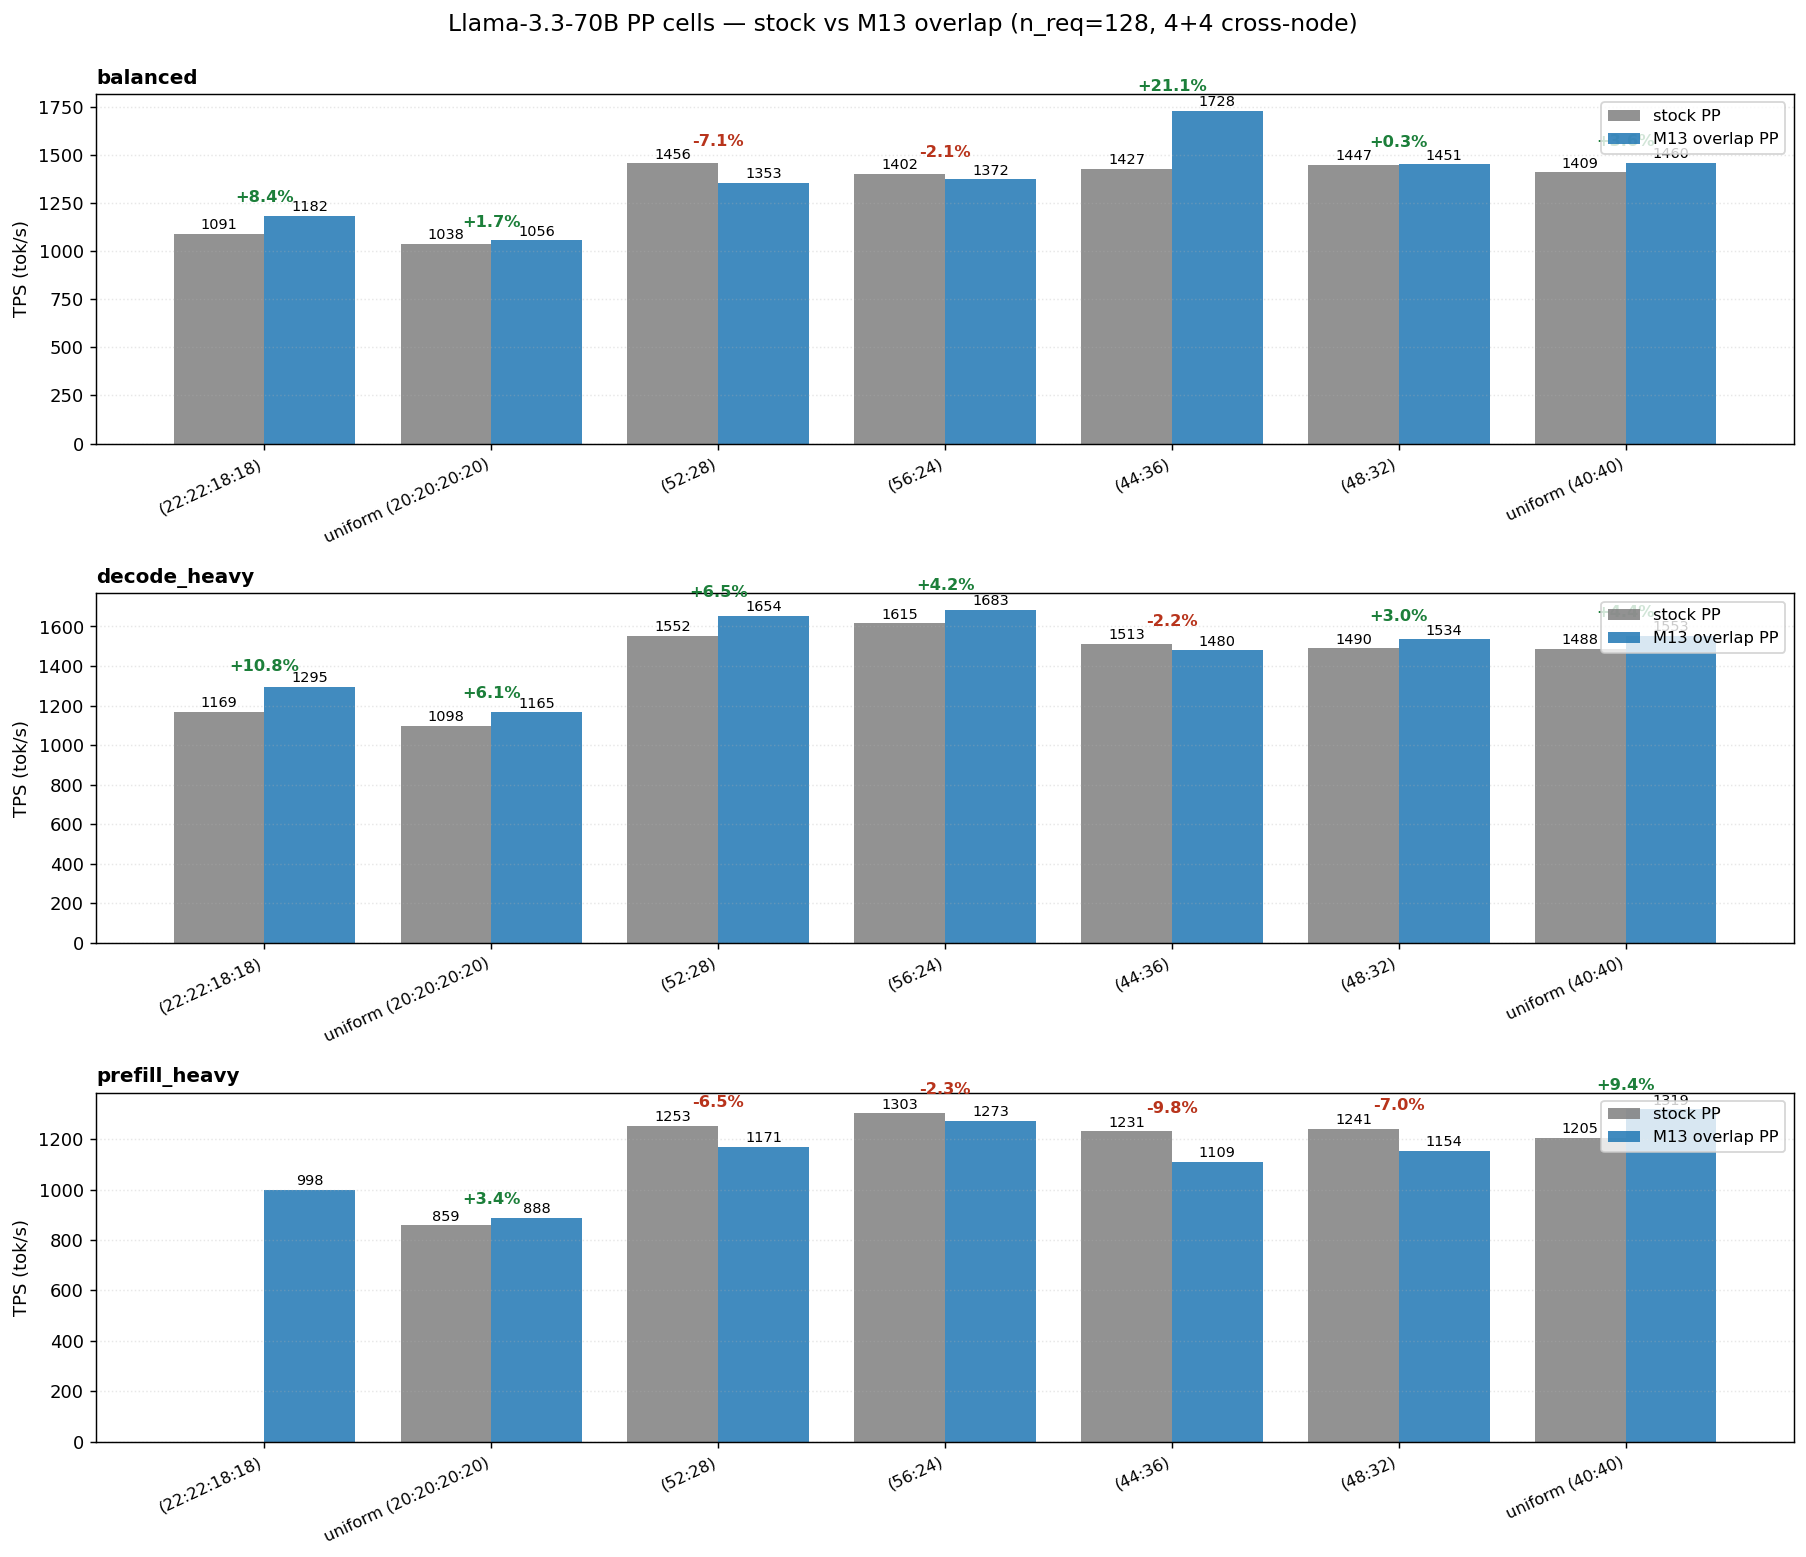
\includegraphics[width=\columnwidth]{figures/fig_70b_stock_vs_overlap.png}
\caption{Stock vs.\ overlap-fixed PP across 70B layer-split configurations ($n_{\text{req}}{=}128$, cross-node). Uniform cells show a clean positive gain; skewed cells are noisier.}
\label{fig:overlap}
\end{figure}

\subsection{Non-uniform Tensor and Pipeline Splits}
\label{sec:eval-nonuniform}

On top of the topology choice, non-uniform partitioning adds a further $+5\%$ to $+25\%$. Table~\ref{tab:ffnbias} and Figure~\ref{fig:ffnbias} sweep FFN bias on the 70B TP8 stage. The benefit is workload-dependent and V-shaped: prefill-heavy gains most ($+18.5\%$ at the $+50\%$-bias point), because prefill is compute-bound and the bias shifts FFN work onto the faster GPUs; decode gains only $+4.3\%$, because at cross-node TP8 the step is dominated by the all-reduce latency floor and the unsplittable attention/KV term, not by FFN weight streaming. The sweet spot lies at $+25$ to $+50\%$ bias and degrades beyond, exactly as the water-filling equalizer predicts (the attention floor on the slow rank cannot be reduced by FFN bias). For the MHA model (OPT-30B), where KV read scales with the head count, biasing \emph{heads} rather than FFN columns is the stronger lever and produces the decode champion. Uneven PP layer allocation is equally important: on the deep TP1$\times$PP8 layout, skewing layers toward the faster node ($14{:}6$ per 4-GPU pair) improves 70B throughput by up to $+51\%$ over a uniform $10{:}10$ split, by lowering the slowest-stage time that bounds the pipeline.

\begin{table}[t]
\centering
\small
\setlength{\tabcolsep}{4pt}
\caption{Non-uniform FFN bias on Llama-3.3-70B, TP8$\times$PP1. Entries are wall throughput (tok/s); bias is the extra FFN columns given to the faster GPUs.}
\label{tab:ffnbias}
\begin{tabular}{lrrr}
\toprule
FFN bias & balanced & decode & prefill \\
\midrule
uniform   & 1394 & 1468 & 1155 \\
$+25\%$   & 1481 & 1503 & 1285 \\
$+50\%$   & 1462 & \textbf{1532} & \textbf{1369} \\
$+75\%$   & 1403 & 1474 & 1237 \\
\bottomrule
\end{tabular}
\end{table}

\begin{figure}[tb]
\centering
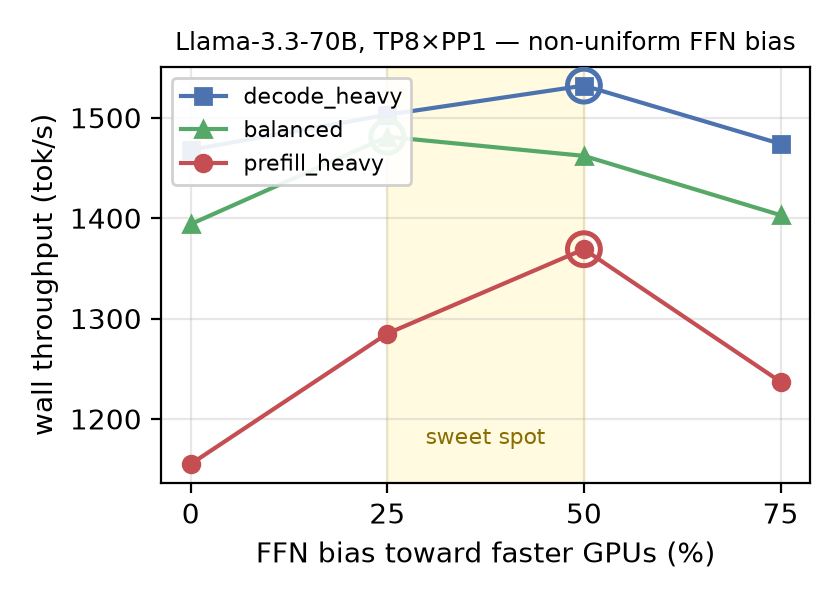
\includegraphics[width=\columnwidth]{figures/fig_70b_ffn_bias.png}
\caption{Non-uniform FFN bias on Llama-3.3-70B (TP8$\times$PP1). Throughput is V-shaped in the bias: it rises to a sweet spot at $+25$ to $+50\%$ (champions circled) and falls beyond, because the slower rank's unsplittable attention/KV floor then bounds the step. Prefill-heavy benefits most ($+18.5\%$); decode least ($+4.3\%$).}
\label{fig:ffnbias}
\end{figure}

\subsection{Planner Accuracy}
\label{sec:eval-planner}

We calibrate the planner on four models (8B, 70B, OPT-30B, Qwen-32B) and evaluate by regret. Across the twelve (model, workload) cells the planner achieves \textbf{mean regret $8.5\%$} (median $7.8\%$, max $28.4\%$), Spearman $\rho{=}0.78$, and a top-3 hit-rate of $3/12$. Exact top-1 champion match is $1/12$, but as argued in Section~\ref{sec:approach-planner} this is noise-limited: the champion and runner-up typically differ by $<5\%$, within measurement noise. Absolute-throughput MAPE ranges from $17\%$ (OPT-30B) to $\sim\!34\%$ (Qwen), i.e.\ the planner ranks configurations well but its magnitude estimate is coarse. Figure~\ref{fig:regret} summarizes the regret distribution and contrasts it with the held-out test below.

\textbf{Pre-registered generalization test.} The strongest evidence for the planner is a held-out, pre-registered prediction. Before any Mistral-Large (123B) measurement existed, we froze the planner's prediction for all three workloads: champion \texttt{TP4$\times$PP2 layer-skew (56:32)} with predicted throughput $805/906/587$ tok/s (balanced/decode/prefill). We then ran the full 45-cell sweep. The result (Table~\ref{tab:mistral}, Figure~\ref{fig:mistral}): \textbf{champion match $3/3$, mean regret $0.0\%$, Spearman $0.84$}. The planner correctly chose the right topology family and the exact champion configuration for a model $1.8\times$ larger than anything in its calibration set, before seeing a single data point. (Its pre-registered caveat---that 123B prefill might prefer TP8 like 70B---did not trigger: Mistral prefill favors PP2, and the planner predicted PP2.) Magnitude was again under-predicted (MAPE $\sim\!32\%$), consistent with the four-model fit; the ranking, which is what plan selection depends on, was correct.

\begin{table}[t]
\centering
\small
\setlength{\tabcolsep}{4pt}
\caption{Pre-registered planner prediction vs.\ measured on the held-out Mistral-Large 123B. Predicted champion was frozen before the sweep. TPS = wall throughput (tok/s).}
\label{tab:mistral}
\begin{tabular}{lrrr}
\toprule
Workload & Pred.\ TPS & Meas.\ TPS & Regret \\
\midrule
balanced       & 805 & 993.8  & $0.0\%$ \\
decode\_heavy  & 906 & 1028.9 & $0.0\%$ \\
prefill\_heavy & 587 & 898.1  & $0.0\%$ \\
\bottomrule
\end{tabular}
\end{table}

\begin{figure*}[t]
\centering

\includegraphics[width=\textwidth]{figures/fig_mistral123b_prereg.png}
\caption{Pre-registered planner prediction (hatched) vs.\ measured (solid) for Mistral-Large 123B across all configurations and three workloads. Champion match $3/3$, mean regret $0.0\%$, Spearman $0.84$.}
\label{fig:mistral}
\end{figure*}

\begin{figure}[tb]
\centering
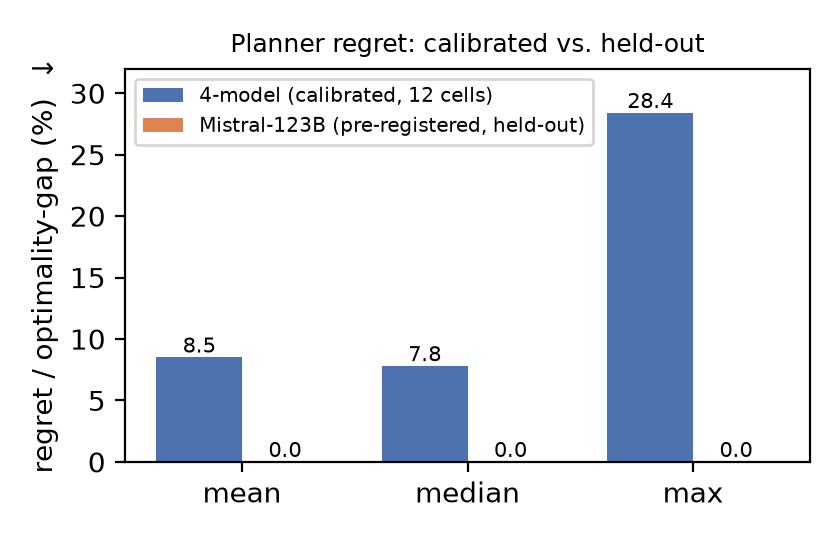
\includegraphics[width=\columnwidth]{figures/fig_planner_regret.png}
\caption{Planner regret (lower is better) on the four calibrated models (12 cells) versus the held-out, pre-registered Mistral-Large 123B. The held-out model incurs $0.0\%$ regret on all three workloads; the calibrated set averages $8.5\%$ (median $7.8\%$) with a $28.4\%$ worst case.}
\label{fig:regret}
\end{figure}

\subsection{Limitations}

Three gaps remain. (1) The planner under-predicts 70B pure-TP8 prefill by $\sim\!2.4\times$; a single global phase-overlap factor $\rho$ cannot simultaneously fit decode/balanced (low $\rho$) and TP8 prefill (which behaves as if prefill is nearly fully hidden), so the planner mis-ranks the one 70B prefill-heavy cell as PP2 instead of TP8 ($15.7\%$ regret on that cell). A per-regime $\rho$ or explicit async-TP modeling would close it. (2) For small models ($\lesssim\!8$B) at cross-node TP8, step time is dispatch/all-reduce-floor bound ($\approx\!48$\,ms floor), which a single global step-floor constant cannot share with the saturated 70B/123B regime; these cells are reported but excluded from the fit. (3) A few Qwen TP8/PP4+ cells are pathological (request preemption/thrash) and were excluded as outliers. None of these affect the headline result: the planner selects the correct topology family in $11/12$ calibrated cells and in $3/3$ held-out cells.

\section{Related Work}

\textbf{LLM serving systems.} Modern serving systems improve throughput through continuous batching, paged KV-cache management, and scheduling. They provide the practical foundation for high-throughput inference but typically assume fixed parallelism or homogeneous hardware when selecting TP/PP layouts. Our engine is built as a fork of such a system and adds non-uniform partitioning and a decode-path overlap fix.

\textbf{Tensor and pipeline parallelism.} TP and PP are standard for distributed training and inference; prior work studies their trade-off but mostly under uniform partitioning across identical devices. We instead allocate uneven tensor shards and uneven layers jointly, driven by per-device profiles.

\textbf{Heterogeneous LLM inference.} Recent work serves LLMs on heterogeneous clusters via device placement, quantization, memory-aware scheduling, or phase-aware execution. We differ by treating non-uniform hybrid TP/PP \emph{planning} as the problem---jointly selecting intra-layer shards and inter-layer allocation from hardware and workload profiles---and by validating an analytical planner with a pre-registered prediction.

\textbf{Prefill--decode disaggregation and phase-aware scheduling.} Several systems observe that prefill and decode have different resource profiles and schedule them separately. We apply the same insight to model-parallel \emph{planning}: the serving phase changes not only request scheduling but the best TP/PP degree and non-uniform split.

\section{Conclusion}

We studied workload-aware non-uniform hybrid parallelism for LLM inference on a real heterogeneous GPU cluster. Uniform TP and PP are insufficient when device capabilities differ, because they create rank-level stragglers and stage-level bottlenecks, and the best configuration depends on the serving workload. Across five models and three workloads we showed that a pipelined hybrid layout with skewed layers wins by up to $+155\%$ over uniform TP, but that prefill-heavy 70B instead prefers pure non-uniform TP---``hybrid is not always best.'' We identified and fixed a decode-path synchronization gate that raises pipeline overlap from $12$--$24\%$ to $56$--$78\%$ with bit-identical outputs, the precondition for hybrid layouts to win, and showed that non-uniform TP/PP splits add a further $+5$ to $+25\%$. Finally, we proposed an analytical planner that selects the full non-uniform hybrid layout from a roofline model and a $\le 6$-cell calibration, achieving $8.5\%$ mean regret on four calibrated models and $0.0\%$ regret on a pre-registered, held-out 123B model. Together these results offer a practical path toward efficient LLM inference on heterogeneous GPU clusters.

\end{document}
